\documentclass[12pt]{report}
\usepackage{amsmath}
\usepackage{graphicx}
\usepackage{hyperref}
\usepackage[utf8]{inputenc}
\usepackage{pgfplots}

\title{ST3009 Weekly Questions 4}
\author{Séamus Woods \\ 15317173}
\date{25/02/2019}

\begin{document}
\maketitle
\newpage

\section{Question 1}
Consider an experiment where we roll two 6-sided dice. Let random variable $Y$ be the sum of the values rolled. The sample space is $\{(1,1),(1,2),(1,3),...,(6,6)\}$ and recall that a random event is a subset of the sample space.
\newline
\newline
(a) What random event corresponds to $Y = 2$?
\newline
The only event where the sum of the values rolled will be two, is when both dice are 1. So the random event that corresponds to $Y = 2$ is $\{(1,1)\}$
\newline
\newline
(b) What event corresponds to $Y = 3$?
\newline
The event that corresponds to $Y = 3$ is $\{(1,2),(2,1)\}$.
\newline
\newline
(c) What event corresponds to $Y = 4$?
\newline
The even that corresponds to $Y = 4$ is $\{(1,3),(2,2),(3,1)\}$.
\newline
\newline
(d) Now let $X$ be the indicator random variable associated with the event $\{(1,1),(2,2),(3,3)\}$. What is the probability that $X = 1$?
\newline
An indicator random variable will take the value 1 if event E occurs, and 0 if event E does not occur. So the probability that our indicator random variable will be 1, is the probability that any of the following will occer (1,1), (2,2), (3,3). We know the sample space is 36..(6*6) and $\frac{3}{36} = 0.0833$.


\section{Question 2}
Let $X$ represent the difference between the number of heads and the number of tails obtained when a coin is tossed 3 times. 
\newline
\newline
(a) What are the possible values of $X$ ?
\newline
If a coin is tossed three times, the amount of possibilities we have is $2^3 = 8$. These possibilities include (H,H,H), (H,H,T), (H,T,H), (H,T,T), (T,H,H), (T,H,T), (T,T,H) and (T,T,T). Given that a Head is 1 and a Tail is -1, we can sub our values in to work out all the possible values of $X$. $\{(1+1+1), (1+1-1), (1-1+1), (1-1-1), (-1+1+1), (-1+1-1), (-1-1+1), (-1-1-1)\}$ or $\{3, 1, 1, -1, 1, -1, -1, -3\}$ We can ignore duplicate values in the set, so our possible values of $X = \{3,1,-1,-3\}$
\newline
\newline
(b) What is $P(X = -3)$ ?
\newline
$X = -3$ if all values are tails. The chances of this are $\frac{1}{8} = 0.125$
\newline
\newline
(c) What is $P(X = -1)$ ?
\newline
$X = -1$ if exactly one of the tosses are heads. the amount of possibilities of this are $3 \choose 1 $ $* 1^2 = 3$. Therefore the probability of this is $\frac{3}{8} = 0.375$
\newline
\newline
(d) If the coin is assumed fair, calculate the PMF and CDF of $X$ and plot a sketch of both. 
\newline
The PMF of $X$ can be seen below:
\begin{center}
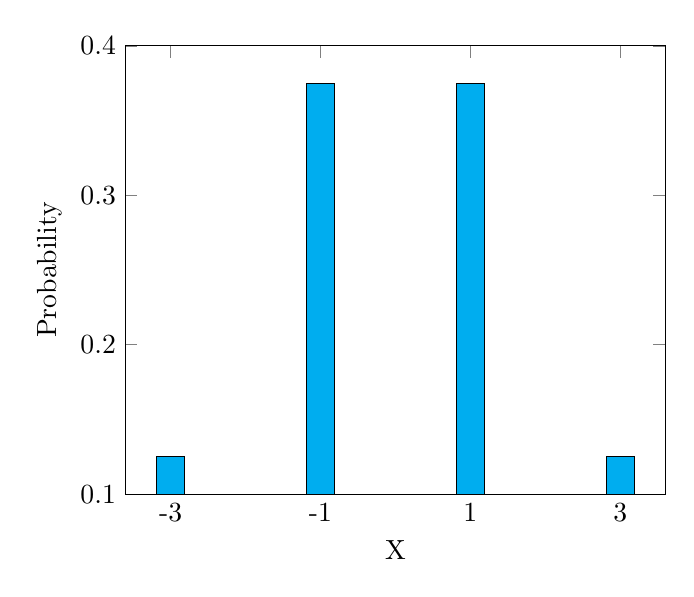
\begin{tikzpicture}
\begin{axis}[
	symbolic x coords = {-3, -1, 1, 3},
	ylabel = {Probability},
	xlabel = {X},
	xtick=data]
\addplot[ybar, fill=cyan] coordinates  {(-3, 0.125) (-1, 0.375) (1, 0.375) (3, 0.125)};
\end{axis}
\end{tikzpicture}
\end{center}
\newpage
The CDF of $X$ can be seen below:
\begin{center}
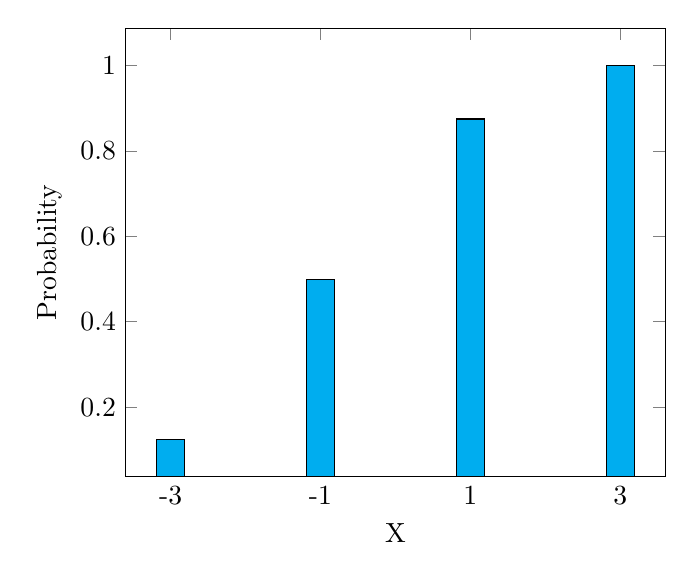
\begin{tikzpicture}
\begin{axis}[
	symbolic x coords = {-3, -1, 1, 3},
	ylabel = {Probability},
	xlabel = {X},
	xtick=data]
\addplot[ybar, fill=cyan] coordinates  {(-3, 0.125) (-1, 0.5) (1, 0.875) (3, 1)};
\end{axis}
\end{tikzpicture}
\end{center}


\section{Question 3}
Four 6-sided dice are rolled. The dice are fair, so each one has equal probability of producing a value in $\{1,2,3,4,5,6\}$. Let $X$ = the minimum of the four values rolled. (It is fine if more than one of the dice has the minimal value.)
\newline
\newline
(a) What is $P(X \geq 1)$ ?
\newline
This is common sense, the probability that $X \geq 1$ = 1, because the minimum possible value is 1, and the chances that the minimum value will be at least that or greater is certain. 
\newline
\newline
(b) What is $P(X \geq 2)$ ?
\newline
The possibility that our minimum value of the four rolls will only hold true if there isn't a single 1 in any of those rolls. Basically this is the probability that there won't be a 1 in any of the four rolls. This can be calculated by rolling anything but a 1 ($\frac{5}{6}$) to the poer of every roll ($4$).. $\frac{5}{6}^4 = 0.4822$  
\newline
\newline
\newpage
(c) What is the CDF of $X$ i.e $P(X \leq k)$ for all values of $k$ ?
\newline
\newline
So we know what $P(X \geq 1)$ and $P(X \geq 2)$ are, we just need to continue this process. $P(X \geq 3)$ should be the probability that there are no 1's plus the probability that there are no 2's, so $\frac{4}{6}^4 = 0.1975$. Continuing this with $P(X \geq 4) = \frac{3}{6}^4 = 0.0625$. $P(X \geq 5) = \frac{2}{6}^4 = 0.01234$. $P(X \geq 6) = \frac{1}{6}^4 = 0.00077$. Using this information we can now find out the probabilities that $P(X \leq k)$. For example we know that the $P(X \leq 1)$ is just $1 - P(X \geq 2) = 1 - 0.4822 = 0.5178$. $P(X \leq 2)$ is the probability that the minimum number is less or equal to two, meaning the minimum number is either 1 or 2 \textbf{or} $1 - P(X \geq 3) = 1 - 0.1975 = 0.8025$. Continuing this process gives us that $P(X \leq 3) = 0.9374$, $P(X \leq 4) = 0.9876$, $P(X \leq 5) = 0.9992$ and $P(X \leq 6) = 1$
\newline
The CDF of $X$ can be seen below:
\newline
\begin{center}
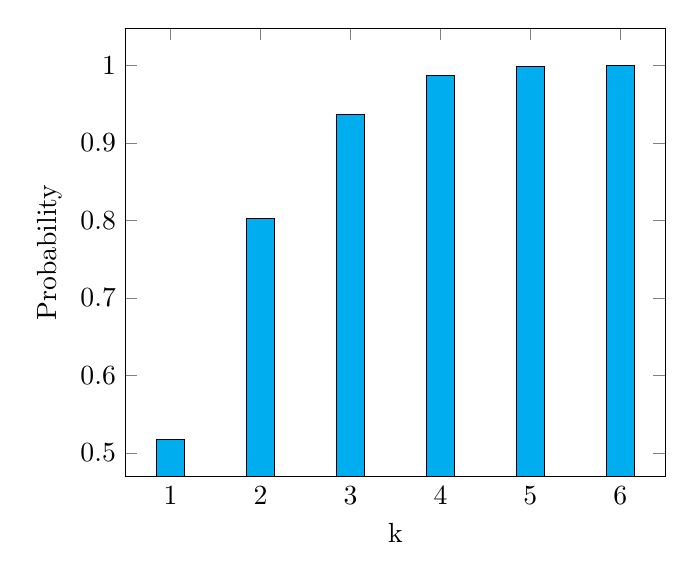
\begin{tikzpicture}
\begin{axis}[
	symbolic x coords = {1,2,3,4,5,6},
	ylabel = {Probability},
	xlabel = {k},
	xtick=data]
\addplot[ybar, fill=cyan] coordinates  {(1,0.5178) (2,0.8025) (3, 0.9374) (4, 0.9876) (5, 0.9992) (6, 1)};
\end{axis}
\end{tikzpicture}
\end{center}

\end{document}